\documentclass[11pt]{article}
 
\usepackage[top=0.75in, bottom=1.25in, left=1in, right=1in]{geometry} 
\usepackage{amsmath,amsthm,amssymb} %this is THE math package
\usepackage{mathtools}
\usepackage{tikz}
\usepackage{graphicx}
\usepackage{fancybox}
\usepackage{hyperref}
\usepackage{varwidth}
\usepackage{mdframed}
\usepackage{mathrsfs}
\usepackage[most]{tcolorbox}
%------------------------
%Fonts I use, uncomment if you like to use them.
%The first is the general font, and the second a math font
\usepackage{mathpazo}
\usepackage{eulervm}
%------------------------
%This is so that we have standard fonts for the double-stroked symbols
%for reals, naturals etc. regardless of what font you use.
%Don't comment
\AtBeginDocument{
  \DeclareSymbolFont{AMSb}{U}{msb}{m}{n}
  \DeclareSymbolFontAlphabet{\mathbb}{AMSb}}
%------------------------
\usepackage{graphicx}
\graphicspath{ {./images/} }

%----------------------------------------------
%User-defined environments
%Commented because we're not using them in this document
%The only uncommented ones are the Problem and Solution environment

% \newenvironment{theorem}[2][Theorem]{\begin{trivlist}
% \item[\hskip \labelsep {\bfseries #1}\hskip \labelsep {\bfseries #2.}]}{\end{trivlist}}
% \newenvironment{lemma}[2][Lemma]{\begin{trivlist}
% \item[\hskip \labelsep {\bfseries #1}\hskip \labelsep {\bfseries #2.}]}{\end{trivlist}}
% \newenvironment{exercise}[2][Exercise]{\begin{trivlist}
% \item[\hskip \labelsep {\bfseries #1}\hskip \labelsep {\bfseries #2.}]}{\end{trivlist}}
% \newenvironment{question}[2][Question]{\begin{trivlist}
% \item[\hskip \labelsep {\bfseries #1}\hskip \labelsep {\bfseries #2.}]}{\end{trivlist}}
% \newenvironment{corollary}[2][Corollary]{\begin{trivlist}
% \item[\hskip \labelsep {\bfseries #1}\hskip \labelsep {\bfseries #2.}]}{\end{trivlist}}
\newenvironment{problem}[2][Problem\!]{\begin{trivlist}
\item[\hskip \labelsep {\bfseries #1}\hskip \labelsep {\bfseries #2}]}{\end{trivlist}}
%\newenvironment{sub-problem}[2][]{\begin{trivlist}
%\item[\hskip \labelsep {\bfseries #1}\hskip \labelsep {\bfseries #2}]}{\end{trivlist}}
\newenvironment{solution}{\begin{proof}[\textbf{\textit{Solution}}] }{\end{proof}}
%----------------------------------------------

%----------------------------
%User-defined notations
\newcommand{\zz}{\mathbb Z}   %blackboard bold Z
\newcommand{\qq}{\mathbb Q}   %blackboard bold Q
\newcommand{\ff}{\mathbb F}   %blackboard bold F
\newcommand{\rr}{\mathbb R}   %blackboard bold R
\newcommand{\nn}{\mathbb N}   %blackboard bold N
\newcommand{\cc}{\mathbb C}   %blackboard bold C
\newcommand{\af}{\mathbb A}   %blackboard bold A
\newcommand{\pp}{\mathbb P}   %blackboard bold P
\newcommand{\id}{\operatorname{id}} %for identity map
\newcommand{\im}{\operatorname{im}} %for image of a function
\newcommand{\dom}{\operatorname{dom}} %for domain of a function
\newcommand{\cat}[1]{\mathscr{#1}}   %calligraphic category
\newcommand{\abs}[1]{\left\lvert#1\right\rvert} %for absolute value
\newcommand{\norm}[1]{\left\lVert#1\right\rVert} %for norm
\newcommand{\modar}[1]{\text{ mod }{#1}} %for modular arithmetic
\newcommand{\set}[1]{\left\{#1\right\}} %for set
\newcommand{\setp}[2]{\left\{#1\ \middle|\ #2\right\}} %for set with a property
\newcommand{\card}[1]{\#\,{#1}} %for cardinality of a set
\newcommand\m[1]{\begin{pmatrix}#1\end{pmatrix}} 

%Re-defined notations
\renewcommand{\epsilon}{\varepsilon}
\renewcommand{\phi}{\varphi}
\renewcommand{\emptyset}{\varnothing}
\renewcommand{\geq}{\geqslant}
\renewcommand{\leq}{\leqslant}
\renewcommand{\Re}{\operatorname{Re}}
\renewcommand{\Im}{\operatorname{Im}}
%----------------------------

\allowdisplaybreaks
 
 
\begin{document}
 
\title{11/22 Submission}
\author{Kevin Guillen\\[0.5em]
MATH 101 | Problem Solving | Fall 2021}
\date{} 

\maketitle
%Use \[...\] instead of $$...$$

\begin{tcolorbox}
  \begin{problem} {IC | 11/15 | 148. (Putnam)} 
    A rectangel HOMF, has sides $\abs{\overline{HO}} = 11$ and $\abs{\overline{OM}} = 5$. A triangle $\triangle ABC$ has $H$ as the intersection of the altidudes, $O$ the center of the circum-circle, $M$ the midpoint of $\abs{\overline{BC}}$ and $F$ the foot of hte altitude from $A$. What is the length of $\abs{\overline{BC}}$?
  \end{problem}
\end{tcolorbox}
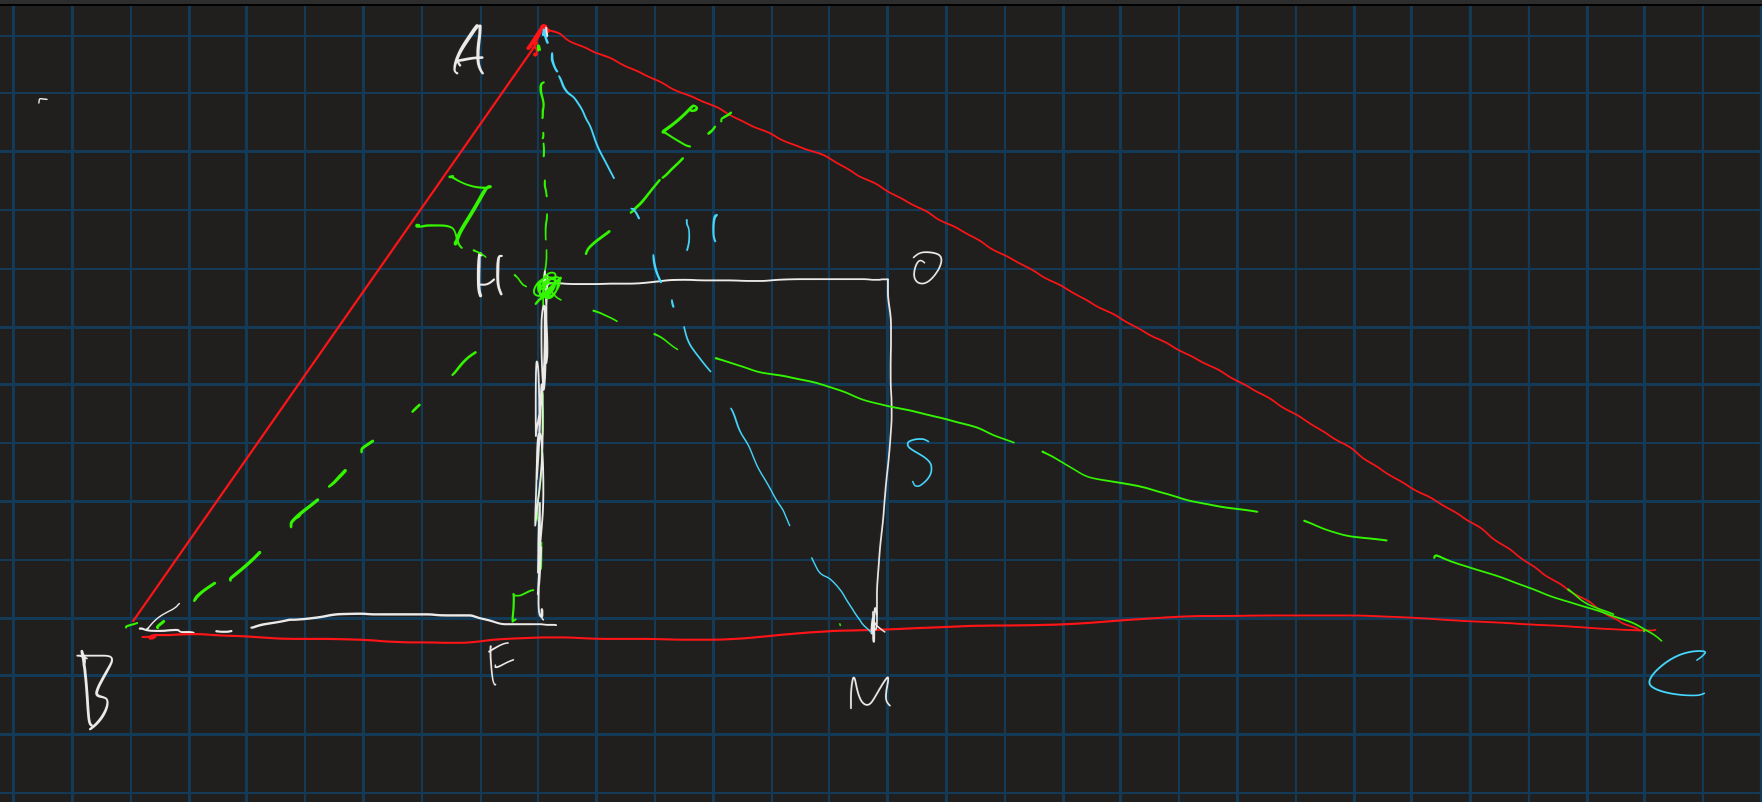
\includegraphics[scale=.5]{prob1}
\begin{proof}
    \newcommand{\leng}[1]{\abs{\overline{#1}}}
    First consider the point $Z$ which is the centroid of of the triangle. We know that $Z$ is colinear to $H$ and $O$. This is noted because the centroid divides the medians into a $2:1$ ratio, and since $H$ and $O$ are colinear with $C$, that means $AH:HF$ has a $2:1$ ratio. Therefore \[\abs{\overline{AF}} = 3 \cdot \leng{HF} = 3 \cdot \leng{OM} = 15.\]

    We can also see that $\triangle BHF$ is similair to $\triangle ACF$, this gives us, \[\frac{\leng{BF}}{\leng{HF}} = \frac{\leng{AF}}{\leng{FC}} \rightarrow \leng{BF} \cdot \leng{FC} = \leng{AF} \cdot \leng{HF}  = 75. \]

    Now consider $\leng{BC}^{2}$, 
    \begin{align*}
        \leng{BC}^{2} &= (\leng{BF} + \leng{FC})^{2} \\
        &= (\leng{BF} - \leng{FC})^{2} + 4\leng{BF}\leng{FC} \\
        &= ((\leng{BM} - \leng{FM}) - (\leng{FM} + \leng{MC}))^{2} + 4\leng{BF}\leng{FC} \\
        &= (-2\leng{FM})^{2} + 4\leng{BF}\leng{FC} && \leng{BM} = \leng{MC} \\
        &= (2\leng{FM})^{2}+ 4\leng{BF}\leng{FC} .
    \end{align*}

    Solving for $\leng{BC}$, we get,
    \begin{align*}
        \leng{BC} &= \sqrt{(2\leng{FM})^{2}+ 4\leng{BF}\leng{FC}} \\
        &= \sqrt{22^{2} + 4(75)} \\
        &= 28.
    \end{align*}

    Thus the length of $\overline{BC}$ is 28.

\end{proof}


\begin{tcolorbox}
    \begin{problem} {IC | 11/15 | 151.}
        Is it possible for a triangle to have altitudes equal to 6, 10, and 20?
    \end{problem}
\end{tcolorbox}
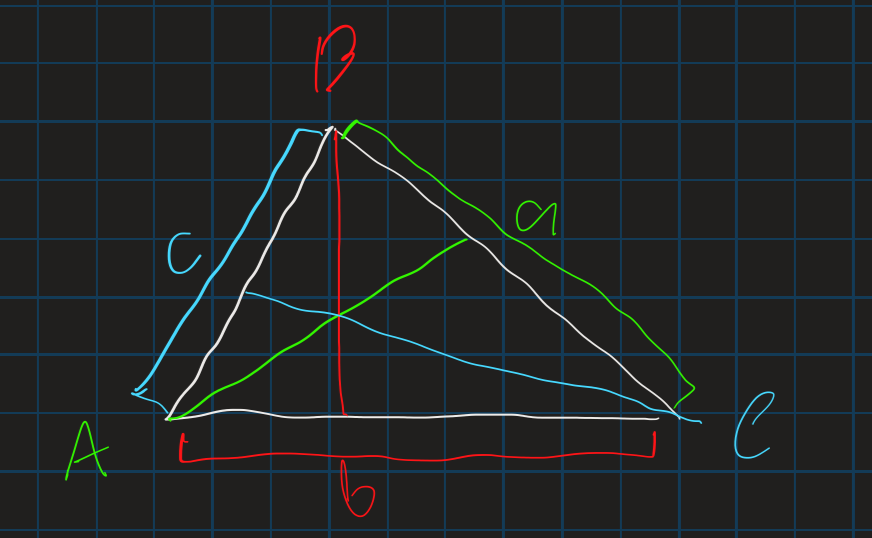
\includegraphics[scale=.5]{prob2}
\begin{proof}
    Consider the area of the triangle drawn above. It will be the following,
    \[A = \frac{6}{2}a = \frac{10}{2}b = \frac{20}{2}c.\]

    Which gives us the following equations,
    \begin{align*}
        a &= \frac{1}{3}A \\
        b &= \frac{1}{5}A \\
        c &= \frac{1}{10}A
    \end{align*}

    Recall though by the triangle inequality we have that $a < b + c$, we see through the following though,
    \begin{align*}
        a &< b + c \\
        \frac{10}{30}A &< \frac{6}{30}A + \frac{3}{10}A = \frac{9}{10}A
    \end{align*}
    that if our altitudes were 6, 10 and 20, that would imply $\dfrac{10}{30}A < \dfrac{9}{10}A$ which is a contradiction. Therefore there can not be a triangle with those given altitudes. 
\end{proof}

\begin{tcolorbox}
    \begin{problem} {IC | 11/17 | 153.}
       Let $P$ be an arbitrary point in the interior of an equilateral triangle. Prove that the sum of the distances of P to the three sides is equal to the altitude of this triangle.
    \end{problem}
\end{tcolorbox}
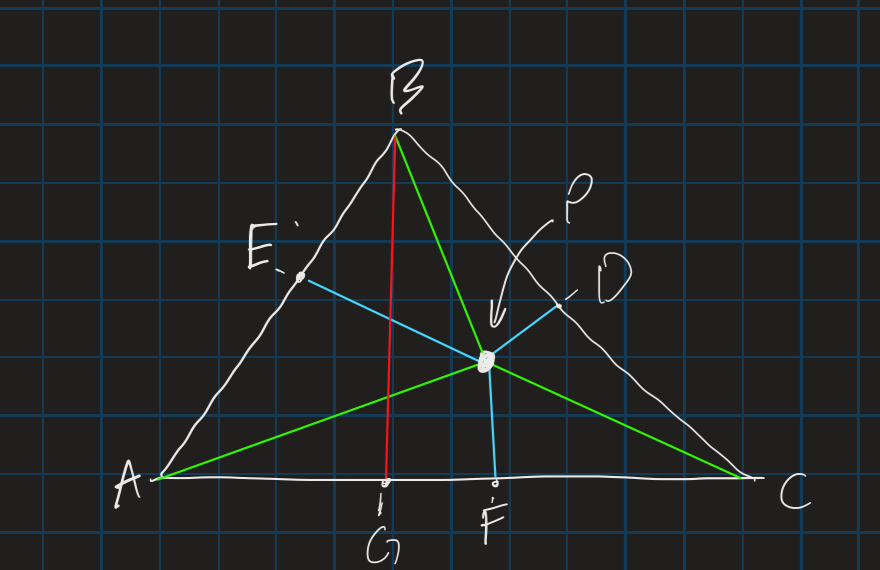
\includegraphics[scale= .5]{prob3}
\begin{proof} \newcommand{\leng}[1]{\abs{\overline{#1}}}
    First let us consider the area of the 3 triangles formed by $P$, 
    \begin{align*}
        [ABP] &= \frac{1}{2} \leng{AB} \cdot \leng{EP} \\
        [BCP] &= \frac{1}{2} \leng{BC} \cdot \leng{DP} \\
        [ACP] &= \frac{1}{2} \leng{AC} \cdot \leng{FP}
    \end{align*}

    These 3 triangles divide $\triangle ABC$ into 3 triangles, therefore the area of $\triangle ABC$ can be obtained by,
    \[[ABC] = [ABP] + [BCP] + [ACP]\]
    Recall though we are working with an equilateral triangle therefore all sides have the same length, which we can denote as $L$. This gives us,
    \begin{align*}
        [ABC] = \frac{1}{2} L \cdot (\leng{EP} + \leng{DP} +\leng{FP}).
    \end{align*}

    We also know though that the area of the triangle can be obtained by $[ABC] = \dfrac{1}{2} L \cdot \leng{BG}$. We see though $\overline{BG}$ is the alitude of the triangle, giving us, 
    \begin{align*}
        \frac{1}{2} L \cdot (\leng{EP} + \leng{DP} +\leng{FP}) &= \frac{1}{2} L \cdot \leng{BG} \\
        \leng{EP} + \leng{DP} +\leng{FP} &= \leng{BG}
    \end{align*}
    as desired.
\end{proof}
\newpage
\begin{tcolorbox}
    \begin{problem} {OC | 11/01 | 68}
        Imagine an $n \times n$ chessboard. How many ways is it possible to choose four squares, no three in the same row or columns which are the vertices of a rectangle?
    \end{problem}
\end{tcolorbox}
\begin{proof}
    If we have an $n\times n$ chessboard that means we have $n$ columns and $n$ rows. We can treat each row and column as sides of a rectangles. If we choose 2 unique vertical lines and 2 unique horizontal lines their intersections will generate a rectangle. There are n choose 2 ways to pick our horizontal lines, and n choose 2 ways to pick our vertical lines This means for an $n \times n$ chessboard we have, 
    \[\binom{n}{2}\binom{n}{2}\]
    rectangles

\end{proof}
\begin{tcolorbox}
    \begin{problem} {OC | 11/01 | 72.}
        How many ways are there to arrange 5 red balls, 7 green balls, and 9 blue balls in a line such that there are never two consecutive white balls?
    \end{problem}
\end{tcolorbox}

\begin{proof}
    The problem mentions no white balls so I'm just going to choose how many ways are there such that there are never two consecutive blue balls.

    First we can line up the red and green balls to have a total line of 12 balls. Then we have 12 choose 7 ways to arrange the 7 green balls in this line of 12. This line of 12 will create 13 spaces, where 2 spaces at the ends of the line and 11 spaces between consecutive balls. This gives us 13 choose 9 ways to insert the blue balls into these spaces such that there are never 2 consecutive blue balls. This gives us,
    \[\binom{12}{7}\binom{13}{9} = 566280\]
\end{proof}

\begin{tcolorbox}
    \begin{problem} {OC | 11/03 | 77.}
        A poker hand consists of five cards. How many poker hands have a card from each of the four suits?
    \end{problem}
\end{tcolorbox}
\begin{proof}
    In this situation there has to be a suit that appears twice in the hand and the rest appear once. There are 4 ways to choose which suit will appear twice and then there are 13 choose 2 ways to pick 2 cards from the suit. Then there are 13 ways to pick a card for each of the remaining 3 suits. This gives us,
    \[4 \cdot \binom{13}{2} \cdot 13 \cdot 13 \cdot 13 = 685464. \]

    So there are 685464 hands that contain at least 1 of each suit.
\end{proof}

\begin{tcolorbox}
    \begin{problem} {OC | 11/08 | 82.}
        Let $p$ be a prime. If $0 < k < p$ prove that $p$ divides $\binom{p}{k} $
    \end{problem}
\end{tcolorbox}
\begin{proof}
    By definition we know $p$ choose $k$ to be,
    \begin{align*}
        \binom{p}{k} &= \frac{p!}{k!(p-k)!} \\
        &= \frac{(p\cdot  \dots \cdot 2 \cdot 1)}{ (k\cdot  \dots \cdot 2\cdot 1)((p-k)\cdot \dots 2 \cdot 1)}
    \end{align*}

    We know though the above will be an integer, but $k, (p-k) < p$, and the only factors of $p$ are $1$ and $p$. We see $p$ is in the numerator and $p$ there is nothing in the denominator to cancel it out. Thus $p$ choose $k$ is indeed dividible by $p$ for $0 < k < p$.
\end{proof}

\begin{tcolorbox}
    \begin{problem} {OC | 11/08 | 83.}
        Prove that consecutive fibonacci nubers are relatively prime.
    \end{problem}
\end{tcolorbox}
\begin{proof}
    We know $F(1) = 1$ and $F(2) = 2$, thus, GCD$(F(1), F(2)) = 1$. 
    
    Assume that GCD$(F(n), F(n+1)) = 1$ holds.
    
    Now consider GCD$(F(n+1), F(n+2)) = $ GCD$(F(n+1), F(n+1) + F(n))$, but this is will be the same as GCD$(F(n+1), F(n))$, but from our induction step this is $1$.

    Therefore any two consecutive fibonacci terms are relatively prime.
\end{proof}

\begin{tcolorbox}
    \begin{problem} {OC | 11/10 | 86.}
        Prove that there are no positive integers $x$, $y$ such that $x+y$, $2x + y$, and $x + 2y$ are squares. 
    \end{problem}
\end{tcolorbox}
\begin{proof}
    Assuming this were to be true, then for integers $a$, $b$, and $c$ we have,
    \begin{align*}
        x+y &= a^{2} \\
        2x+y &= b^{2} \\
        x + 2y &= c^{2}
    \end{align*}
    Using the 2nd equation to solve for $y$ we get, $y = b^{2} -2x$. Plugging this into the 1st equation we get, $x = b^{2} - a^{2}$. Using the 1st equation to solve for $x$ we get, $x = a^{2} -y$. Pluggin this into the 2nd equation we get $y = 2a^{2} -b^{2}$.

    Now plugging in these value into the 3rd equation, we get,
    \begin{align*}
        a^{2}-y + 4a^{2} -2b^{2} &= c^{2} \\
        3a^{2} &= b^{2} + c^{2}
    \end{align*}

    Thus there is only integer solutions if this diophantine equation holds. We know any integers squared mod 4 will have values 0 or 1. Therfore $b^{2} + c^{2} \in \set{0,1,2}$, and $3a^{2}\in \set{0,3}$. This together means we must have $3a^{2} \equiv 0 \text{ mod } 4$ and $(b^{2} + c^{2}) \equiv 0 \text{ mod }4$. Meaning $a$ is even and is of the form $a = 2k$, also means that $b$ and $c$ are even and of the form $b = 2l$ and $c = 2n$. Plugging this back into the equation we get,
    \begin{align*}
        12k^{2} & = 4l^{2} + 4n^{2}.
    \end{align*}

    This means there has to be a solution for $k$, $l$, and $n$. But this can be since $k + l + n < a + b + c$. Therefore there is no integers $x$ and $y$ such that $x +y$, $2x +y$, and $x + 2y$ are squares.
\end{proof}


\begin{tcolorbox}
    \begin{problem} {OC | 11/15 | 97.}
        Let $P$ be a point inside a circle such that there are three chords through $P$ of equal length. Prove that $P$ is the center of the circle.
    \end{problem}
\end{tcolorbox}
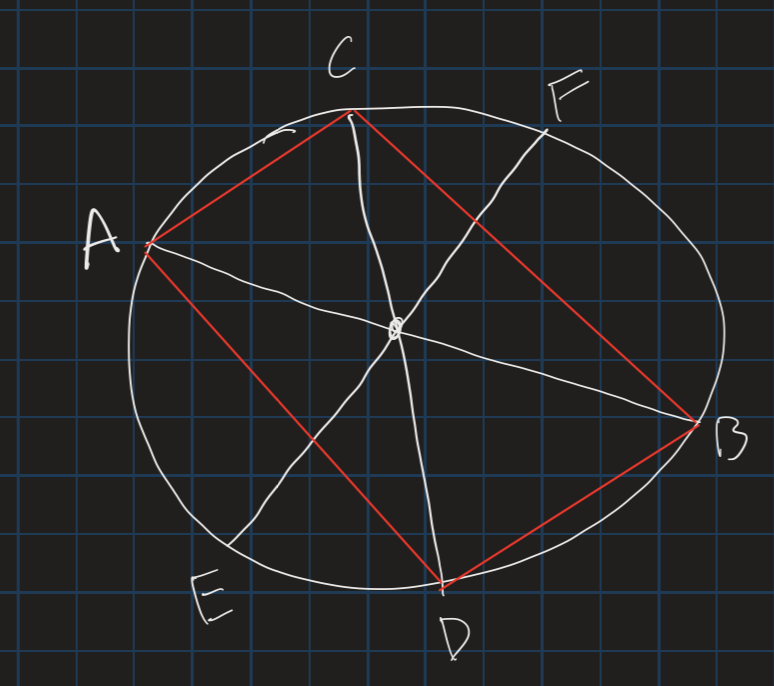
\includegraphics[scale=.5]{prob4}
\begin{proof}
    Let $\overline{AB}$, $\overline{CD}$, and $\overline{EF}$, represent the 3 chords of equal length that intersect at $P$. Consider the two chords $\overline{AB}$ and $\overline{CD}$. We know we can create a parallelogram from $ACBD$, where $\angle ACD = \angle DBC$ and $\angle ACD = \angle ABD$, all this together the parallelogram is actually a rectangle. Which means the circle is the circumscribing circle of this rectangle. The the diagonals of $ACBD$ which were $\overline{AB}$ and $\overline{CD}$ actually have length diameter. Since $P$ is the intersection of these two diameters $P$ must be the center of the circle. 
\end{proof}

\end{document}